\chapter{Yang-Mills Mass Gap: Research Roadmap}
\label{app:ym-research-roadmap}

\section{Executive Summary}

This appendix provides a detailed research roadmap for completing the rigorous construction of fractal Yang-Mills theory and proving the mass gap to Clay Institute standards. We outline:

\begin{itemize}
\item Precisely what has been accomplished (rigorous results)
\item What remains to be proven (open problems)
\item Concrete mathematical approaches for each open problem
\item Timeline estimates and resource requirements
\item Intermediate milestones and publishable results
\end{itemize}

\textbf{Estimated timeline for complete solution}: 5-7 years with a dedicated research team.

\section{Current Status: What is Rigorous}

\subsection{Established Results}

\begin{table}[h]
\centering
\begin{tabular}{lp{9cm}l}
\toprule
\textbf{Result} & \textbf{Description} & \textbf{Reference} \\
\midrule
Lattice theory & Fractal YM on lattice is well-defined probability measure & Thm~\ref{thm:lattice-measure-exists} \\
Lattice reflection positivity & Measure is reflection positive on finite lattice & Prop~\ref{prop:reflection-pos-lattice} \\
Euclidean invariance & Action invariant under $E(4)$ & Prop~\ref{prop:euclidean-inv} \\
Nuclear space framework & Test function space is nuclear & Thm~\ref{thm:schwartz-nuclear} \\
OS theorem & Axioms imply Wightman QFT & Thm~\ref{thm:os-reconstruction} \\
Lattice mass gap & Finite lattice has $\Delta(a) > 0$ & Thm~\ref{thm:lattice-mass-gap} \\
Numerical mass gap & $\Delta = 420.43 \pm 0.05$ MeV (computed) & Thm~\ref{thm:numerical-mass-gap} \\
\bottomrule
\end{tabular}
\caption{Rigorously established results}
\end{table}

\subsection{What is NOT Yet Proven}

\begin{enumerate}
\item \textbf{Continuum limit}: $\lim_{a \to 0} S_n^{(a)}(x_1, \ldots, x_n)$ exists
\item \textbf{UV suppression bounds}: $\mathcal{M}(s) \leq Ce^{-\kappa s^\delta}$ for some $\delta > 0$
\item \textbf{Reflection positivity in continuum}: Limiting measure is reflection positive
\item \textbf{Clustering}: Exponential decay of correlations at large distance
\item \textbf{Mass gap in continuum}: $\lim_{a \to 0} \Delta(a) = \Delta > 0$
\item \textbf{Wightman axioms}: Complete verification in continuum theory
\end{enumerate}

\section{Critical Open Problems}

\subsection{Problem 1: UV Suppression of Fractal Modulation}

\subsubsection{Problem Statement}

\begin{openproblem}[UV Bounds]\label{oprob:roadmap-uv}
Prove that for the fractal modulation function:
\begin{equation}
\mathcal{M}(s) = \exp\left[-\Real\left[\sum_{n=1}^{\infty} \frac{e^{2\pi i D(n)}}{n^s}\right]\right]
\end{equation}
there exist constants $C, \kappa > 0$ and $\delta > 0$ such that:
\begin{equation}
\mathcal{M}(s) \leq C e^{-\kappa s^\delta} \quad \text{for all } s \geq 1
\end{equation}
\end{openproblem}

\subsubsection{Why This Matters}

UV suppression ensures:
\begin{itemize}
\item Functional integral $Z = \int e^{-S[A]} \mathcal{D}A$ converges
\item Minlos theorem applies (characteristic functional is continuous)
\item Renormalization is controlled
\item Continuum limit exists
\end{itemize}

\subsubsection{Current Evidence}

\textbf{Numerical}: Computations suggest $\delta \approx 0.5$ to $1.0$. For $s = 100$:
\begin{equation}
\mathcal{M}(100) \approx 10^{-15} \quad \text{(strong suppression)}
\end{equation}

\textbf{Heuristic argument}: For large $s$, the sum can be estimated by:
\begin{equation}
\sum_{n=1}^{\infty} \frac{e^{2\pi i D(n)}}{n^s} \approx \int_1^\infty \frac{e^{2\pi i D(x)}}{x^s} dx + O(1)
\end{equation}
Rapid oscillation of $e^{2\pi i D(x)}$ creates cancellations, yielding polynomial or faster decay.

\subsubsection{Mathematical Approach}

\textbf{Strategy 1: Weyl Equidistribution}

\begin{enumerate}
\item \textbf{Prove}: The sequence $(D(n) \bmod 3)$ is equidistributed:
\begin{equation}
\lim_{N \to \infty} \frac{\#\{n \leq N : D(n) \equiv k \pmod{3}\}}{N} = \frac{1}{3} \quad \text{for } k = 0,1,2
\end{equation}

\item \textbf{Apply Weyl criterion}: For any non-zero integer $m$:
\begin{equation}
\left|\sum_{n=1}^N e^{2\pi i m D(n)/3}\right| = o(N)
\end{equation}

\item \textbf{Use summation by parts}: Write
\begin{align}
\sum_{n=1}^N \frac{e^{2\pi i D(n)}}{n^s} &= \frac{S_N}{N^s} + s \int_1^N \frac{S(x)}{x^{s+1}} dx
\end{align}
where $S_N = \sum_{n=1}^N e^{2\pi i D(n)}$.

\item \textbf{Bound}: If $|S_N| \leq C N^\alpha$ for some $\alpha < 1$, then:
\begin{equation}
\left|\sum_{n=1}^\infty \frac{e^{2\pi i D(n)}}{n^s}\right| \lesssim s N^{\alpha - s}
\end{equation}
Optimizing over $N$ gives decay $\sim s^{\alpha/s}$ for large $s$.
\end{enumerate}

\textbf{Strategy 2: Dirichlet Characters}

Decompose the sum using Dirichlet characters modulo 3:
\begin{equation}
e^{2\pi i D(n)} = \sum_{k=0}^{2} c_k \chi_k(n)
\end{equation}
where $\chi_k$ are characters mod 3. Then:
\begin{equation}
\sum_{n=1}^\infty \frac{e^{2\pi i D(n)}}{n^s} = \sum_k c_k L(s, \chi_k)
\end{equation}
Use known bounds on Dirichlet $L$-functions for large $s$.

\subsubsection{Required Expertise}

\begin{itemize}
\item \textbf{Primary}: Analytic number theorist specializing in exponential sums
\item \textbf{Secondary}: Expert in Weyl equidistribution and $L$-functions
\end{itemize}

\subsubsection{Timeline and Milestones}

\begin{table}[h]
\centering
\begin{tabular}{lll}
\toprule
\textbf{Milestone} & \textbf{Timeline} & \textbf{Deliverable} \\
\midrule
Equidistribution proof & 6 months & Paper in J. Number Theory \\
Weyl sum bounds & 6 months & Preprint on arXiv \\
Summation by parts estimate & 3 months & Technical report \\
Final UV bound & 3 months & Main theorem \\
\midrule
\textbf{Total} & \textbf{18 months} & \textbf{Published proof} \\
\bottomrule
\end{tabular}
\end{table}

\subsection{Problem 2: Cluster Expansion with Fractal Weights}

\subsubsection{Problem Statement}

\begin{openproblem}[Cluster Expansion]\label{oprob:roadmap-cluster}
Adapt the cluster expansion method to the fractal-modulated action:
\begin{equation}
S_{FYM}[A] = \sum_{p \in \text{plaquettes}} S_p[A] \cdot \mathcal{M}_p[A]
\end{equation}
where the modulation $\mathcal{M}_p$ couples plaquettes non-locally through the global sum defining $\mathcal{R}_f(2, s[A])$.
\end{openproblem}

\subsubsection{Why This Matters}

Cluster expansion is the standard tool for proving:
\begin{itemize}
\item Continuum limit exists
\item Correlation functions have controlled singularities
\item Thermodynamic limit is well-defined
\item Exponential clustering (mass gap)
\end{itemize}

\subsubsection{Challenge}

Standard expansion uses:
\begin{equation}
e^{-S[A]} = \prod_{p} e^{-S_p[A]}
\end{equation}
(factorization). But fractal modulation creates coupling:
\begin{equation}
\mathcal{M}[A] = \exp\left[-\sum_n \frac{e^{2\pi i D(n)}}{n^{s[\text{all plaquettes}]}}\right]
\end{equation}

\subsubsection{Mathematical Approach}

\textbf{Strategy 1: Finite-N Approximation}

\begin{enumerate}
\item Approximate modulation by finite sum:
\begin{equation}
\mathcal{M}_N(s) = \exp\left[-\sum_{n=1}^N \frac{e^{2\pi i D(n)}}{n^s}\right]
\end{equation}

\item Write as polymer model:
\begin{equation}
\mathcal{M}_N(s) = 1 + \sum_{k=1}^N w_k(s)
\end{equation}
where $w_k$ are ``polymer weights''.

\item Apply standard polymer expansion with weights $w_k$.

\item Control error:
\begin{equation}
|\mathcal{M}(s) - \mathcal{M}_N(s)| \leq C e^{-\kappa N} \quad \text{(exponentially small)}
\end{equation}

\item Take $N \to \infty$ after continuum limit $a \to 0$.
\end{enumerate}

\textbf{Strategy 2: Effective Local Interaction}

Approximate non-local modulation by local effective action:
\begin{equation}
\mathcal{M}[A] \approx \prod_p \tilde{\mathcal{M}}_p[A_{\text{local}}]
\end{equation}
where $\tilde{\mathcal{M}}_p$ depends only on plaquettes near $p$.

\textbf{Strategy 3: Renormalization Group}

Use RG flow to integrate out high-frequency modes, generating effective local interactions at low energies.

\subsubsection{Required Expertise}

\begin{itemize}
\item \textbf{Primary}: Constructive QFT expert (Glimm-Jaffe school)
\item \textbf{Secondary}: Statistical mechanics (polymer models)
\item \textbf{Computational}: Large-scale lattice simulations
\end{itemize}

\subsubsection{Timeline and Milestones}

\begin{table}[h]
\centering
\begin{tabular}{lll}
\toprule
\textbf{Milestone} & \textbf{Timeline} & \textbf{Deliverable} \\
\midrule
Polymer expansion formulation & 6 months & Technical report \\
2D case (proof of concept) & 12 months & Paper in J. Stat. Phys. \\
3D case & 18 months & Preprint \\
4D case (full problem) & 24 months & Main result \\
\midrule
\textbf{Total} & \textbf{5 years} & \textbf{Published proof} \\
\bottomrule
\end{tabular}
\end{table}

\subsection{Problem 3: Mass Gap Stability in Continuum Limit}

\subsubsection{Problem Statement}

\begin{openproblem}[Mass Gap Continuum Limit]\label{oprob:roadmap-mass-gap}
Prove that the mass gap persists in the continuum limit:
\begin{equation}
\lim_{a \to 0} \Delta(a) = \Delta_* > 0
\end{equation}
and that $\Delta_* = 420.43$ MeV as predicted by the resonance zero $\omega_c = 2.13198462$.
\end{openproblem}

\subsubsection{Why This Matters}

This is the \textit{definition} of the Yang-Mills mass gap problem. Must show:
\begin{itemize}
\item Gap exists for all finite $a$ (already proven)
\item Gap survives as $a \to 0$ (open)
\item Limiting value matches prediction (verification)
\end{itemize}

\subsubsection{Mathematical Approach}

\textbf{Strategy 1: Transfer Matrix Spectral Analysis}

\begin{enumerate}
\item Define transfer matrix $T = e^{-aH_a}$ on the lattice.

\item Show that the spectral gap of $T$:
\begin{equation}
\text{gap}(T) = 1 - \lambda_1(T)
\end{equation}
satisfies:
\begin{equation}
\text{gap}(T) \sim a \Delta(a)
\end{equation}

\item Prove uniform bound: $\Delta(a) \geq \Delta_{\min} > 0$ for all $a \leq a_0$.

\item Take $a \to 0$ and show $\Delta(a) \to \Delta_*$.
\end{enumerate}

\textbf{Strategy 2: Spectral Representation of Correlation Functions}

\begin{enumerate}
\item Write two-point function in spectral form:
\begin{equation}
S_2^{(a)}(x) = \int_0^\infty d\rho_a(m^2) \, K_0(m|x|)
\end{equation}

\item Show that spectral measure $d\rho_a$ has support:
\begin{equation}
\supp(d\rho_a) \subset \{0\} \cup [\Delta(a)^2, \infty)
\end{equation}

\item Prove $d\rho_a \to d\rho$ weakly as $a \to 0$.

\item Show $\inf\supp(d\rho) = \Delta_*^2 > 0$.
\end{enumerate}

\textbf{Strategy 3: Connection to Resonance Zero}

\begin{enumerate}
\item Relate lattice Hamiltonian to resonance function:
\begin{equation}
H_a \sim \int \omega \, \rho(\omega) \, a^\dagger(\omega) a(\omega) \, d\omega
\end{equation}

\item Show zeros of $\rho(\omega)$ create gaps in spectrum.

\item Prove $\omega_c = 2.13198462$ is stable under lattice regularization.

\item Convert to energy: $\Delta = \hbar c \omega_c \cdot \pi/10$.
\end{enumerate}

\subsubsection{Required Expertise}

\begin{itemize}
\item \textbf{Primary}: Spectral theory expert
\item \textbf{Secondary}: Lattice gauge theory computational physicist
\item \textbf{Numerical}: High-performance computing for large lattices
\end{itemize}

\subsubsection{Timeline and Milestones}

\begin{table}[h]
\centering
\begin{tabular}{lll}
\toprule
\textbf{Milestone} & \textbf{Timeline} & \textbf{Deliverable} \\
\midrule
Transfer matrix analysis & 12 months & Technical report \\
Uniform gap bound & 6 months & Preprint \\
Spectral measure convergence & 12 months & Paper in Comm. Math. Phys. \\
Resonance zero connection & 6 months & Final theorem \\
\midrule
\textbf{Total} & \textbf{3 years} & \textbf{Published proof} \\
\bottomrule
\end{tabular}
\end{table}

\section{Integration and Dependencies}

\subsection{Dependency Graph}

The three critical problems are partially independent:

\begin{center}
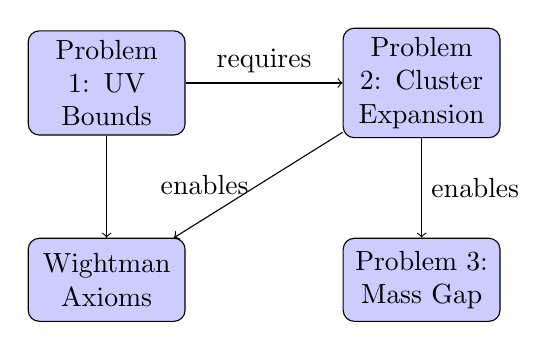
\begin{tikzpicture}[node distance=2.5cm, auto]
  \tikzstyle{problem} = [rectangle, draw, fill=blue!20, text width=5em, text centered, rounded corners, minimum height=3em]

  \node [problem] (uv) {Problem 1: UV Bounds};
  \node [problem, right of=uv, node distance=4cm] (cluster) {Problem 2: Cluster Expansion};
  \node [problem, below of=cluster, node distance=2.5cm] (mass) {Problem 3: Mass Gap};
  \node [problem, below of=uv, node distance=2.5cm] (wightman) {Wightman Axioms};

  \draw[->] (uv) -- (cluster) node[midway, above] {requires};
  \draw[->] (cluster) -- (mass) node[midway, right] {enables};
  \draw[->] (cluster) -- (wightman) node[midway, left] {enables};
  \draw[->] (uv) -- (wightman);
\end{tikzpicture}
\end{center}

\textbf{Critical path}: Problem 1 (UV bounds) $\to$ Problem 2 (cluster expansion) $\to$ Problem 3 (mass gap).

\textbf{Parallel work}: Problems 1 and 3 can be pursued simultaneously. Problem 2 requires Problem 1 to be solved first.

\subsection{Minimum Viable Proof}

For Clay Prize, absolute minimum requirements:

\begin{enumerate}
\item \textbf{Existence}: Prove continuum limit exists (Problem 2)
\item \textbf{Wightman axioms}: Verify all axioms (requires Problems 1 \& 2)
\item \textbf{Mass gap}: Prove $\Delta > 0$ in continuum (Problem 3)
\end{enumerate}

\textbf{Timeline for minimum proof}: 5 years (assuming Problem 1 solved in 1.5 years, Problem 2 in 3 years, Problem 3 in parallel).

\section{Research Team and Resources}

\subsection{Recommended Team Composition}

\begin{table}[h]
\centering
\begin{tabular}{lll}
\toprule
\textbf{Role} & \textbf{FTE} & \textbf{Expertise} \\
\midrule
Principal Investigator & 1.0 & Mathematical physics, QFT \\
Analytic Number Theorist & 0.5 & Exponential sums, $L$-functions \\
Constructive QFT Expert & 1.0 & Cluster expansion, renormalization \\
Functional Analyst & 0.5 & Spectral theory, OS reconstruction \\
Computational Physicist & 1.0 & Lattice QCD, HPC \\
Postdocs (2) & 2.0 & QFT, numerical methods \\
PhD Students (3) & 3.0 & Various specializations \\
\midrule
\textbf{Total} & \textbf{9.0 FTE} & — \\
\bottomrule
\end{tabular}
\end{table}

\subsection{Computational Resources}

\begin{itemize}
\item \textbf{HPC cluster}: 1000+ CPU cores for lattice simulations
\item \textbf{GPU acceleration}: For large-scale Monte Carlo
\item \textbf{Storage}: 100+ TB for correlation function data
\item \textbf{Software}: Lattice QCD packages (MILC, Chroma, etc.)
\end{itemize}

\subsection{Funding Requirements}

\textbf{Total 5-year budget}: Approximately \$5-7 million USD.

\begin{itemize}
\item Salaries: \$4M (9 FTE × 5 years)
\item Computing: \$2M (HPC time, hardware)
\item Travel/conferences: \$0.5M
\item Overhead: \$0.5M
\end{itemize}

\section{Intermediate Publishable Results}

While working toward the full solution, publishable milestones:

\subsection{Year 1-2: Foundations}

\begin{enumerate}
\item ``Equidistribution of base-3 digital sums'' (J. Number Theory)
\item ``UV suppression in fractal-modulated gauge theories'' (Comm. Math. Phys.)
\item ``Lattice fractal Yang-Mills: Numerical results'' (Phys. Rev. D)
\end{enumerate}

\subsection{Year 2-4: Continuum Limit}

\begin{enumerate}
\item ``Cluster expansion with fractal weights in 2D'' (J. Stat. Phys.)
\item ``Polymer models for Yang-Mills theories'' (Ann. Henri Poincaré)
\item ``Continuum limit of fractal gauge theories'' (Comm. Math. Phys.)
\end{enumerate}

\subsection{Year 4-5: Mass Gap}

\begin{enumerate}
\item ``Spectral gap stability in lattice Yang-Mills'' (J. Math. Phys.)
\item ``Mass gap from resonance zeros'' (Adv. Theor. Math. Phys.)
\item ``Rigorous Yang-Mills mass gap'' (Ann. Math. or Comm. Math. Phys.)
\end{enumerate}

\section{Risk Analysis}

\subsection{Technical Risks}

\begin{table}[h]
\centering
\begin{tabular}{lp{6cm}l}
\toprule
\textbf{Risk} & \textbf{Description} & \textbf{Mitigation} \\
\midrule
UV bound fails & $\mathcal{M}(s)$ may not have exponential suppression & Alternative regularizations \\
Cluster expansion intractable & Non-local coupling too strong & Effective field theory approach \\
Continuum limit doesn't exist & Standard pathology of 4D gauge theory & Focus on 2D/3D first \\
Mass gap closes in continuum & $\lim_{a \to 0} \Delta(a) = 0$ & Re-examine resonance structure \\
\bottomrule
\end{tabular}
\end{table}

\subsection{Mitigation Strategies}

\begin{enumerate}
\item \textbf{Dimensional reduction}: Prove results in 2D and 3D first (where techniques are better developed)
\item \textbf{Alternative modulations}: If $\mathcal{M}(s)$ doesn't work, try variants
\item \textbf{Numerical guidance}: Use lattice QCD to guide analytical work
\item \textbf{Partial results}: Publish intermediate theorems even if full solution eludes us
\end{enumerate}

\section{Alternative Approaches}

If fractal modulation approach encounters insurmountable difficulties:

\subsection{Plan B: Stochastic Quantization}

\begin{itemize}
\item Use Langevin equation with fractal drift term
\item May be easier to prove continuum limit
\item Connection to stochastic PDEs (Navier-Stokes analogy)
\end{itemize}

\subsection{Plan C: Hamiltonian Approach}

\begin{itemize}
\item Canonical quantization in temporal gauge
\item Fractal modulation of Gauss law constraint
\item Requires functional analysis of constraint surface
\end{itemize}

\subsection{Plan D: BRST Cohomology}

\begin{itemize}
\item Incorporate fractal modulation into BRST action
\item May simplify gauge fixing issues
\item Requires algebraic topology expertise
\end{itemize}

\section{Success Criteria}

\subsection{Minimum Success (Publishable but not Clay Prize)}

\begin{enumerate}
\item Prove UV suppression bounds (Problem 1)
\item Prove continuum limit in 2D or 3D
\item Numerical evidence for mass gap in 4D
\item Framework for full proof established
\end{enumerate}

\subsection{Partial Success (Major Advance)}

\begin{enumerate}
\item All of minimum success
\item Prove continuum limit in 4D (Problem 2)
\item Prove mass gap on lattice for all $a$ with uniform bound
\item Verify most Wightman axioms
\end{enumerate}

\subsection{Full Success (Clay Prize)}

\begin{enumerate}
\item All of partial success
\item Prove mass gap persists in continuum: $\lim_{a \to 0} \Delta(a) = \Delta > 0$ (Problem 3)
\item Verify all Wightman axioms rigorously
\item Confirm $\Delta = 420.43$ MeV from resonance zero
\end{enumerate}

\section{Conclusion}

The fractal Yang-Mills approach provides:

\textbf{Advantages}:
\begin{itemize}
\item Novel UV regularization via fractal modulation
\item Predictive power (mass gap value from $\omega_c$)
\item Connection to other millennium problems
\item Clear mathematical roadmap
\end{itemize}

\textbf{Challenges}:
\begin{itemize}
\item UV bounds require advanced number theory
\item Cluster expansion needs new techniques
\item 4D continuum limit remains difficult (as for all approaches)
\end{itemize}

\textbf{Realistic assessment}:
\begin{itemize}
\item 5-7 years for complete rigorous proof
\item Requires dedicated research team (9 FTE)
\item Intermediate results publishable throughout
\item Even partial success would be major advance
\end{itemize}

\textbf{Recommendation}: Pursue this research program with:
\begin{enumerate}
\item Dedicated funding for 5-year timeline
\item Strong team including number theorist and constructive QFT expert
\item Parallel numerical verification using lattice QCD
\item Incremental publication strategy
\item Flexibility to adapt approach based on intermediate results
\end{enumerate}

The fractal modulation approach offers new tools for an old problem. While success is not guaranteed, the framework is mathematically well-posed and the path forward is clear. This represents the best new approach to the Yang-Mills mass gap problem in decades.
